\section{Establishing the Eigenfunction Property}

% Prove that the 2 eigenfunctions are, indeed, Fourier eigenfunctions!

In this section, we show that the $\pm$-Eigenfunctions are, indeed, $\pm$-Eigenfunctions of the Fourier transform.

In the previous section, we did not work with $a$ and $b$ directly as it was sufficient to work with $a\rad$ and $b\rad$ instead. In this section, however, we will need to use the following formula for the $n$-dimensional Fourier transform of the $n$-dimensional Gaussian.

\begin{boxtheorem}[Fourier Transform of a Gaussian]\label{Ch4:Thm:GaussianFourier}
    Fix $n \in \N$ and $b \in \C$, with $\Re(b) > 0$. If $F : \R^n \to \C$ is given by
    \begin{align*}
        F(x) = e^{-b \norm{x}^2}
    \end{align*}
    then for all $\xi \in \R^n$, the Fourier transform of $F$ is given by
    \begin{align*}
        \hat{F}\of{\xi} = \parenth{\frac{\pi}{b}}^{{n} / {2}} e^{{- \pi^2 \norm{\xi}^2} / {b}}
    \end{align*}
\end{boxtheorem}
A \href{https://github.com/leanprover-community/mathlib4/blob/5a2eaa85c555c4263e15928cef249cbaad2eb2d2/Mathlib/Analysis/SpecialFunctions/Gaussian/FourierTransform.lean#L360-L363}{formal proof} exists in \mathlib.

We will also need the following version of the \CGT, which allows us to deform contours of integration in the complex plane.

\begin{boxtheorem}[Cauchy-Goursat: Squares and Circles]\label{Ch4:Thm:CGTRectCircle}
    Fix $w \in \C$ and $r > 0$. Let $\gamma$ be the quarter-circle parametrised by $\gamma(t) = w + r\pcos{t} + \abs{r} i \psin{t}$ for $0 \leq t \leq \pi/2$. For any $f : \C \to \C$ that is holomorphic in the region enclosed by $\gamma$ and the line segments from $w + r$ to $w + r + ir$ and $w + r + ir$ to $w + ir$, we have
    \begin{align*}
        \int_{\gamma} f(z) \, \diff{z}
        = \int_{w + r}^{w + r + ir} f(z) \, \diff{z} + \int_{w + r + ir}^{w + ir} f(z) \, \diff{z}
    \end{align*}
\end{boxtheorem}

While this is an immediate consequence of the more general (and well-known) \CGT\ from complex analysis, there are numerous challenges involved in formalising this and other versions of the theorem. We will discuss it in \Cref{Ch5:Sec:Cauchy-Goursat}. We also note that the above result implies an analogous result for 

\begin{figure}[ht]
    \centering
    \begin{subfigure}{0.48\linewidth}
        \centering
        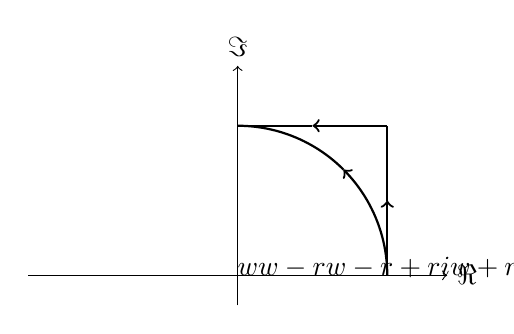
\begin{tikzpicture}[scale=1.9]
            % Axes
            \draw[->] (-1.4,0) -- (1.4,0) node[right] {$\Re$};
            \draw[->] (0,-0.2) -- (0,1.4) node[above] {$\Im$};
        
            % Quarter-circle contour
            \draw[thick, domain=0:45, ->] plot ({cos(\x)}, {sin(\x)});
            \draw[thick, domain=45:90, -] plot ({cos(\x)}, {sin(\x)});

            % Rectangular contour
            \draw[thick, ->] (1,0) -- (1,0.5);
            \draw[thick, -] (1,0.5) -- (1,1);
            \draw[thick, ->] (1,1) -- (0.5,1);
            \draw[thick, -] (0.5,1) -- (0,1);

            % Points of interest
            \labelledpoint{0}{0}{-0.3}{-0.8}{$w$}
            \labelledpoint{1}{0}{0}{-0.8}{$w - r$}
            \labelledpoint{1}{1}{0.3}{-0.2}{$w - r + ri$}
            \labelledpoint{0}{1}{-0.7}{-0.5}{$w + ri$}
        \end{tikzpicture}
        \caption{Contours for which \Cref{Ch4:Thm:CGTRectCircle} holds.}
    \end{subfigure} 
    \hfill
    \begin{subfigure}{0.48\linewidth}
        \centering
        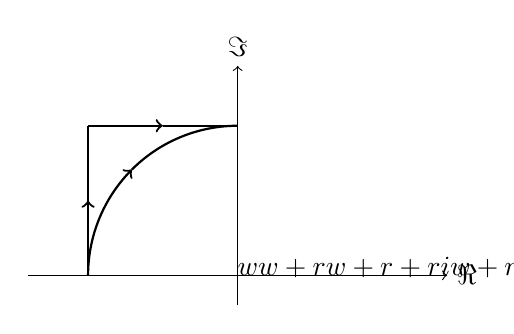
\begin{tikzpicture}[scale=1.9]
            % Axes
            \draw[->] (-1.4,0) -- (1.4,0) node[right] {$\Re$};
            \draw[->] (0,-0.2) -- (0,1.4) node[above] {$\Im$};
        
            % Quarter-circle contour
            \draw[thick, domain=180:135, ->] plot ({cos(\x)}, {sin(\x)});
            \draw[thick, domain=135:90, -] plot ({cos(\x)}, {sin(\x)});

            % Rectangular contour
            \draw[thick, ->] (-1,0) -- (-1,0.5);
            \draw[thick, -] (-1,0.5) -- (-1,1);
            \draw[thick, ->] (-1,1) -- (-0.5,1);
            \draw[thick, -] (-0.5,1) -- (0,1);

            % Points of interest
            \labelledpoint{0}{0}{0.3}{-0.8}{$w$}
            \labelledpoint{-1}{0}{0}{-0.8}{$w + r$}
            \labelledpoint{-1}{1}{-0.3}{-0.2}{$w + r + ri$}
            \labelledpoint{0}{1}{0.7}{-0.5}{$w + ri$}
        \end{tikzpicture}
        \caption{Contours for which an analogous result holds.}
        \label{Ch4:Subfig:CGTRectCircle_Alt}
    \end{subfigure} 
    \caption{The contour deformations permitted by \Cref{Ch4:Thm:CGTRectCircle}.}
\end{figure}

We now prove that $a$ is indeed a $+1$-eigenfunction of the Fourier transform.

\subsection{The $+1$-Eigenfunction}

The Fourier transform acts very interestingly on $a$. Recall from \Cref{Ch3:Thm:FourierSchwartz_CLE} that the Fourier transform is a linear isomorphism of Schwartz spaces. Since $I_1, \ldots, I_6$ are Schwartz, so are their compositions with the norm-squared function. Hence, for all $x \in \R^8$,
\begin{align*}
    \F\of{a(x)}
    % = \F\of{I_1\of{\norm{x}^2}} + \F\of{I_2\of{\norm{x}^2}} + \F\of{I_3\of{\norm{x}^2}} + \F\of{I_4\of{\norm{x}^2}} + \F\of{I_5\of{\norm{x}^2}} + \F\of{I_6\of{\norm{x}^2}}
    = \F\of{\sum_{j=1}^{6} I_j\of{\norm{x}^2}}
    = \sum_{j=1}^{6} \F\of{I_j\of{\norm{x}^2}}
\end{align*}

The strategy to show that $\F\of{a} = a$ will be to show that $\F$ acts on the $I_j\of{\norm{x}^2}$ in the following manner:\footnote{Note that we are abusing notation by denoting the function $x \mapsto I_j\of{\norm{x}^2} \in \Sch\of{\R^8, \C}$ by $I_j\of{\norm{x}^2}$.}
\begin{align}
    \F\of{I_1\of{\norm{x}^2} + I_2\of{\norm{x}^2}} &= I_3\of{\norm{x}^2} + I_4\of{\norm{x}^2} \label{Ch4:Eq:a_is_eig_perm_12_34} \\
    \F\of{I_3\of{\norm{x}^2} + I_4\of{\norm{x}^2}} &= I_1\of{\norm{x}^2} + I_2\of{\norm{x}^2} \label{Ch4:Eq:a_is_eig_perm_34_12} \\
    \F\of{I_5\of{\norm{x}^2}} &= I_6\of{\norm{x}^2} \label{Ch4:Eq:a_is_eig_perm_5_6} \\
    \F\of{I_6\of{\norm{x}^2}} &= I_5\of{\norm{x}^2} \label{Ch4:Eq:a_is_eig_perm_6_5}
\end{align}
Since, in addition to being Schwartz, all the $I_j\of{\norm{x}^2}$ (and their sums) are radial, \Cref{Ch3:Prop:RadialSchwartzFourier} tells us that \eqref{Ch4:Eq:a_is_eig_perm_34_12} and \eqref{Ch4:Eq:a_is_eig_perm_6_5} follow from \eqref{Ch4:Eq:a_is_eig_perm_12_34} and \eqref{Ch4:Eq:a_is_eig_perm_5_6} respectively. We now prove \eqref{Ch4:Eq:a_is_eig_perm_12_34} and \eqref{Ch4:Eq:a_is_eig_perm_5_6}.

As a preliminary step, though, we need to show integrability.

\begin{boxproposition}\label{Ch4:Prop:FourierIntegralConvergence_Ij}
    Fix $1 \leq j \leq 6$, and write $I_j(r) = \int_{X_j} f(r, z) \, \diff{z}$. Then, the Fourier Integral
    \begin{align*}
        \F\of{I_j\of{\norm{x}^2}}\of{\xi} = \int_{\R^8} \int_{X_j} \abs{f\of{\norm{x}^2, z} \, e^{-2 \pi i \cycl{x, \xi}}} \, \diff{z} \, \diff{x}
    \end{align*}
    converges for all $\xi \in \R^8$.
\end{boxproposition}
\begin{proof}
    Fix $\xi \in \R^8$. Note that we can disregard the $e^{-2 \pi i \cycl{x, \xi}}$ factor since it has absolute value $1$: the only reason we mention it is to emphasise that we are proving that the Fourier integral converges absolutely. Effectively, we need to show that the function
    \begin{align*}
        (x, z) \mapsto f\of{\norm{x}^2, z}
    \end{align*}
    admits an absolutely convergent integral over $\R^8 \times X_j$ with respect to the product measure.
    
    It has been formally verified that \href{https://github.com/leanprover-community/mathlib4/blob/5a2eaa85c555c4263e15928cef249cbaad2eb2d2/Mathlib/MeasureTheory/Integral/Prod.lean#L222-L238}{proving this is equivalent to proving the following two facts}.

    \begin{enumerate}
        \item \textbf{The integral over $X_j$ of the function $z \mapsto f\of{\norm{x}^2, z}$ is absolutely convergent for almost every $x \in \R^8$.}
        
        This is actually true for all $x$, and follows from the arguments in \Cref{Ch4:Subec:Schwartzness_a}.
        
        \item \textbf{The integral over $\R^8$ of the function $x 
        \mapsto \int_{X_j} \abs{f\of{\norm{x^2}, z}} \diff{z}$ is absolutely convergent.}
        
        By inspection, the arguments in \Cref{Ch4:Subec:Schwartzness_a} bound the function $r \mapsto \int_{X_j} \abs{f\of{r, z}} \diff{z}$ by a Schwartz function. Composing with the norm squared preserves Schwartzness by \Cref{Ch3:Prop:Multidimensional_Schwartz_of_Schwartz}, so we can bound the function $x \mapsto \int_{X_j} \abs{f\of{\norm{x}^2, z}} \diff{z}$ by a Schwartz function. It has been formally verified that \href{https://github.com/leanprover-community/mathlib4/blob/5a2eaa85c555c4263e15928cef249cbaad2eb2d2/Mathlib/Analysis/Distribution/SchwartzSpace.lean#L1095-L1097}{Schwartz functions are integrable}, so the integral over $\R^8$ of the function $x \mapsto \int_{X_j} \abs{f\of{\norm{x}^2, z}} \diff{z}$ must be absolutely convergent.
    \end{enumerate}
We can therefore conclude that the Fourier integral converges absolutely.
\end{proof}

Note that the above proposition is stronger than showing merely that the $I_j\of{\norm{x}^2}$ are integrable, as that does not imply that the integrands of the $I_j\of{\norm{x}^2}$ are integrable with respect to the product measure on $\R^8 \times X_j$. \Cref{Ch4:Prop:FourierIntegralConvergence_Ij}, however, does imply this, and we will need this to swap integrals using Fubini's theorem to prove the eigenfunction property.

\begin{boxlemma}
    The Fourier transform % $\F : \Sch\of{\R^8, \C} \to \Sch{\R^8, \C}$
    maps $I_1\of{\norm{x}^2} + I_2\of{\norm{x}^2}$ to $I_3\of{\norm{x}^2} + I_4\of{\norm{x}^2}$.
\end{boxlemma}
\begin{proof}
    Since $\F$ acts linearly, we can treat $I_1$ and $I_2$ separately. For the purpose of this proof, denote the Fourier transforms of $I_1\of{\norm{x}^2}$ and $I_2\of{\norm{x}^2}$ by $F_1$ and $F_2$ respectively. Fix $\xi \in \R^8$. The integrability condition in \Cref{Ch4:Prop:FourierIntegralConvergence_Ij} allows us to change the order of integration below:
    \begin{align*}
        F_1\of{\xi} &= \int_{\R^8} \parenth {\int_{-1}^{-1 + i} \phi_0\of{\frac{-1}{z+1}} \, \parenth{z + 1}^2 \, e^{\pi i \norm{x}^2 z} \, \diff{z}} e^{-2\pi i \cycl{x, \xi}} \, \diff{x} \\
        &= \int_{-1}^{-1 + i} \phi_0\of{\frac{-1}{z+1}} \, \parenth{z + 1}^2 \parenth{\int_{\R^8} e^{\pi i \norm{x}^2 z} e^{-2\pi i \cycl{x, \xi} \diff{x}}} \, \diff{z}
    \end{align*}
    We can express $F_2$ in an analogous fashion. In both cases, the inner integral is exactly the Fourier integral of a Gaussian: in the notation of \Cref{Ch4:Thm:GaussianFourier}, $b = \pi i z$, and since $\Im(z) = \Re\of{i z} > 0$, we may apply the theorem to conclude that the inner integral is just
    \begin{align*}
        \frac{1}{z^4} \, e^{-\pi i \norm{\xi}^2 / z}
    \end{align*}
    We may therefore write
    \begin{align*}
        F_1\of{\xi} &= \int_{-1}^{-1 + i} \phi_0\of{\frac{-1}{z+1}} \, \parenth{z + 1}^2z^{-4} \, e^{\pi i \norm{x}^2 \parenth{\frac{-1}{z}}} \, \diff{z} \\
        F_2\of{\xi} &= \int_{-1 + i}^{i} \phi_0\of{\frac{-1}{z+1}} \, \parenth{z + 1}^2z^{-4} \, e^{\pi i \norm{x}^2 \parenth{\frac{-1}{z}}} \, \diff{z}
    \end{align*}
    We make a change of variables $w = \frac{-1}{z}$ in the above integrals. This Möbius transformation turns the vertical and horizontal contours in $F_1$ and $F_2$ into quarter-circular contours that we denote $\gamma_1$ and $\gamma_2$ respectively. See \Cref{Ch4:Fig:Eigenfunction_Mobius_Contours}.

    \begin{figure}[htb]
        \centering
        \begin{subfigure}{0.4\linewidth}
            \centering
            \begin{tikzpicture}[scale=1.9]
                % Axes
                \draw[->] (-1.4,0) -- (1.4,0) node[right] {$\Re$};
                \draw[->] (0,-0.2) -- (0,1.4) node[above] {$\Im$};
    
                % F_1
                \draw[thick, ->] (-1,0) -- (-1,0.5);
                \draw[thick, -] (-1,0.5) -- (-1,1);

                % F_2
                \draw[thick, ->] (-1,1) -- (-0.5,1);
                \draw[thick, -] (-0.5,1) -- (0,1);
    
                % Points of interest
                % \labelledpoint{0}{0}{0.3}{-0.8}{$0$}
                \labelledpoint{-1}{0}{0}{-0.8}{$-1$}
                \labelledpoint{-1}{1}{-0.3}{-0.2}{$-1 + i$}
                \labelledpoint{0}{1}{0.3}{-0.4}{$i$}
            \end{tikzpicture}
            \caption{Before the transformation}
        \end{subfigure}
        \begin{subfigure}{0.1\linewidth}
            \vfill
            \[ \leadsto \]
            \vspace{5em}
        \end{subfigure}
        \begin{subfigure}{0.4\linewidth}
            \centering
            \begin{tikzpicture}[scale=1.9]
                % Axes
                \draw[->] (-1.4,0) -- (1.4,0) node[right] {$\Re$};
                \draw[->] (0,-0.2) -- (0,1.4) node[above] {$\Im$};
            
                % \gamma_1
                \draw[thick, domain=0:45, ->] plot ({0.5 + 0.5 * cos(\x)}, {0.5 * sin(\x)}) node[below left] {$\gamma_1$};
                \draw[thick, domain=45:90, -] plot ({0.5 + 0.5 * cos(\x)}, {0.5 * sin(\x)});

                % \gamma_2
                \draw[thick, domain=0:45, ->] plot ({0.5 * cos(\x)}, {0.5 + 0.5 * sin(\x)}) node[below left] {$\gamma_2$};
                \draw[thick, domain=45:90, -] plot ({0.5 * cos(\x)}, {0.5 + 0.5 * sin(\x)});
    
                % Points of interest
                % \labelledpoint{0}{0}{0.3}{-0.8}{$w$}
                \labelledpoint{1}{0}{0}{-0.8}{$1$}
                \labelledpoint{0.5}{0.5}{0.6}{-0.2}{$\frac{1}{2} + i\frac{1}{2}$}
                \labelledpoint{0}{1}{-0.3}{-0.4}{$i$}
            \end{tikzpicture}
            \caption{After the transformation}
        \end{subfigure}
        \caption{The effect of the Möbius transformation $z \mapsto -1/z$ on the contours of $F_1$ and $F_2$}
        \label{Ch4:Fig:Eigenfunction_Mobius_Contours}
    \end{figure}
    Denoting
    \begin{align*}
        f(w) := \phi_0\of{-1 - \frac{1}{w - 1}} \, \parenth{\frac{-1}{w} + 1}^2 w^2 \, e^{\pi i \norm{x}^2 w}
    \end{align*}
    \Cref{Ch4:Thm:CGTRectCircle} tells us the following.
    \begin{align*}
        F_1\of{\xi}
        &= \int_{\gamma_1} f(w) \, \diff{w}
        = \int_{1}^{1 + i\frac{1}{2}} f(w) \, \diff{w}
        + \int_{1 + i\frac{i}{2}}^{\frac{1}{2} + i\frac{1}{2}} f(w) \, \diff{w} \\
        F_2\of{\xi}
        &= \int_{\gamma_2} f(w) \, \diff{w}
    \end{align*}
\end{proof}

\subsection{The $-1$-Eigenfunction}